\documentclass[a4paper, openany, 14pt]{article}

%% подключаем стандарт библиографии
\bibliographystyle{gost71u}


%% для "Abstract" в классе book
% \newenvironment{abstract}{}{}
% \usepackage{abstract}

%% подключаем преамбулу: в ней содержится подключение всех необходимых пакетов
%% Работа с русским языком
\usepackage{cmap}			 % поиск в PDF
\usepackage{mathtext} 		 % русские буквы в формулах
\usepackage[T2A]{fontenc}	 % кодировка
\usepackage[utf8]{inputenc}	 % кодировка исходного текста
\usepackage[russian]{babel}	 % локализация и переносы

%% Пакеты для работы с математикой
\usepackage{amsmath,amsfonts,amssymb,amsthm,mathtools}
\usepackage{icomma}

%% Нумерация формул (опционально)
%\mathtoolsset{showonlyrefs=true} % показывать номера только у тех формул, на которые есть \eqref{} в тексте.
%\usepackage{leqno}               % нумерация формул слева

%% Шрифты
\usepackage{euscript}	 % шрифт "Евклид"
\usepackage{mathrsfs}    % красивый мат. шрифт

%% Некоторые полезные макросы для дебага (в случае недоверия авторам шаблона)
\makeatletter
\newcommand\thefontsize{The current font size is: \f@size pt} % пример: \section{\thefontsize}
\makeatother

%% Настройка размеров шрифтов
\makeatletter
\setlength{\headheight}{28pt}
%% TODO: мне не удалось разобраться, как грамотно подбирать второе число в 
%% \@setfontsize\*, но ряд эксппериментов показывает, что "10" выравнивает текст весьма прилично :)
\renewcommand\Huge{\@setfontsize\Huge{14pt}{10}}
\renewcommand\huge{\@setfontsize\huge{14pt}{10}}
\renewcommand\Large{\@setfontsize\Large{14pt}{10}}
\renewcommand\large{\@setfontsize\large{14pt}{10}}
\makeatother

%% Поля (геометрия страницы)
\usepackage[left=3cm,right=1.5cm,top=2cm,bottom=2cm,bindingoffset=0cm]{geometry}

%% Русские списки
\usepackage{enumitem}
\makeatletter
\AddEnumerateCounter{\asbuk}{\russian@alph}{щ}
\makeatother

%% Работа с картинками
\usepackage{caption}
\captionsetup{justification=centering} % центрирование подписей к картинкам
\usepackage{graphicx}                  % вставки рисунков
\graphicspath{{images/}{images2/}}     % папки с картинками
\setlength\fboxsep{3pt}                % отступ рамки \fbox{} от рисунка
\setlength\fboxrule{1pt}               % толщина линий рамки \fbox{}
\usepackage{wrapfig}                   % обтекание рисунков и таблиц текстом

%% Работа с таблицами
\usepackage{array,tabularx,tabulary,booktabs} % дополнительная работа с таблицами
\usepackage{longtable}                        % длинные таблицы
\usepackage{multirow}                         % слияние строк в таблице

%% Красная строка
\setlength{\parindent}{2em}

%% Интервалы
\linespread{1}
\usepackage{multirow}

%% TikZ
\usepackage{tikz}
\usetikzlibrary{graphs,graphs.standard}

%% Верхний колонтитул
\usepackage{fancyhdr}
\pagestyle{fancy}

%% Перенос знаков в формулах (по Львовскому)
\newcommand*{\hm}[1]{#1\nobreak\discretionary{}{\hbox{$\mathsurround=0pt #1$}}{}}

%% Дополнительно
\usepackage{float}   % добавляет возможность работы с командой [H] которая улучшает расположение на странице
\usepackage{gensymb} % красивые градусы
\usepackage{caption} % пакет для подписей к рисункам, в частности, для работы caption*
\usepackage{listings} % пакет для листингов с кодом
\lstset{              % настройки для лисингов с кодом
basicstyle=\small\ttfamily,
columns=flexible,
breaklines=true
}

% Hyperref (для ссылок внутри  pdf)
\usepackage[unicode, pdftex]{hyperref}

% Отступ перед первым абзацем в каждом разделе
\usepackage{indentfirst}
    
\usepackage{setspace}
\onehalfspacing


\begin{document}
    %% титульник
    %\begin{center}
    %% *название института*
    \large\textbf{Министерство образования и науки Российской Федерации \\
    Московский физико-технический институт (государственный
    университет)} \\
    \vspace{1cm}

    %% *факультет/физтех-школа*
    Физтех-школа радиотехники и компьютерных технологий \\

    %% *название базовой кафедры и лаборатории*
    %% в случае ненадобности можно удалить
    Кафедра системного программирования ИСП РАН \\
    Лаборатория (laboratory name)\\

    \vspace{3em}

    Выпускная квалификационная работа бакалавра
\end{center}

\begin{center}
    \vspace{\fill}
    %% *название вашей работы*
    \LARGE{Система автоматизированного тестирования файловой системы JFFS2}

    \vspace{\fill}
\end{center}


\begin{flushright}
    \textbf{Автор:} \\
    Студент Б01-009 группы \\
    Дементьев Даниил Викторович \\
    \vspace{2em}
    \textbf{Научный руководитель:} \\
    % *научная степень* \\
    Мутилин Вадим Сергеевич \\
    \vspace{2em}
    \textbf{Научный консультант:} \\
    % *научная степень* \\
    Хорошилов Алексей Владимирович \\
\end{flushright}

\vspace{7em}

\begin{center}
    %% *лого*
    \includegraphics[width=100 pt]{MIPT_logo.jpg}\\
    Москва \the\year{}
\end{center}

%% выключаем отображение номера для этой страницы (титульник)
\thispagestyle{empty}

\newpage
\setcounter{page}{2}
\fancyfoot[c]{\thepage}
%% *надпись над верхним колонтинулом*
%% в случае ненадобности можно удалить
\fancyhead[L]{Система автоматизированного тестирования файловой системы JFFS2}
\fancyhead[R]{}
    %% аннотоция
    \begin{abstract}

    \begin{center}
        \large{Автоматизированная система тестирования файловой системы JFFS2} \\
    \large\textit{Дементьев Даниил Викторович} \\[1 cm]

    Современные операционные системы состоят из множества модулей, реализующих основной функционал для пользователя. Одними из основных являются модули файловых систем, отвечающие за хранение и организацию доступа к пользовательским данным. По оценкам разработчиков, на подгружаемые модули приходится большинство ошибок, приводящих к некорректной работе всей ОС. По этой причине активно разрабатываются системы тестирования модулей ядра Linux с использованием различных подходов к тестированию и анализу кода. В данной работе рассмотрена проблема тестирования файловой системы ядра Linux JFFS2 и описан процесс разработки системы автоматизированного тестирования исследуемой ФС на базе набора регрессионных тестов для различных файловых систем xfstests. В работе рассмотрены основные подходы к тестированию модулей ядра, а также использованы соответствующие различным подходам инструменты. Разработанная система покрывает 79.4\% строк исходного кода JFFS2 и 91.4\% функций. С целью дальнейшего развития разработанной системы в работе проведен анализ непокрытого кода.

    % \newpage

    % \textbf{Abstract} \\[1 cm]

    % Automative JFFS2 filesystem testing suite.
    \end{center}

\end{abstract}
\newpage

    %% содержание
    \tableofcontents{}
    \newpage

    \fontsize{14}{16}\selectfont
    \section{Введение}
\label{sec:Chapter0} \index{Chapter0}

В данной главе вводятся основные понятия, необходимые для постановки задачи.

\subsection{Файловая система}

Одна из основных функций операционной системы (ОС) - управление устройствами долговременного хранения информации и предоставление пользовательским приложениям интерфейса для взаимодействия с ними с целью хранения и организации доступа к данным. Элемент операционной системы, отвечающий за эти функции - \textbf{файловая система} (ФС) \cite{osbook}. 

Для интеграции ряда файловых систем в единую структуру с пользовательской точки зрения в ядре ОС Linux используется концепция виртуальной файловой системы, позволяющая обращаться к различным файловым системам ипользуя единый интерфейс системных вызовов. Для оптимизации своей работы ФС использует множество внутренних структур данных. Для хранения метаданных пользовательских файлов и каталогов ФС использует структуру данных называемую \textbf{индексным дескриптором}. Также для хранения информации о свободном пространстве на устройстве файловые системы используют особые структуры данных, например битовую карту данных или список свободных блоков устройства. Для оптимизации процесса монтирования вся информация о файловой системе необходимая ОС в процессе монтирования хранится в структуре называемой \textbf{суперблоком}.

\subsection{Устройства долговременного хранения информации}

Большинство файловых систем ядра Linux были разработаны для взаимодействия с накопителями на жестком магнитном диске, особенности строения которых формировали алгоритмы хранения данных, используемые файловыми системами. Подобные устройства хранения состоят из вращающегося диска с магнитными дорожками и считывающей головки, способной перемещаться между дорожками. Из-за подобного строения доступ к произвольному блоку данных на жестком диске имел задержку позиционирования считывающей головки над нужной дорожкой и задержку вращения диска, обусловленную скоростью вращения магнитного диска. Для оптимизации задержки вращения в файловых системах использовались различные алгоритмы размещения данных на диске, например размещение файлов из одного каталога и их индексных дескрипторов поблизости.

С развитием технологий на рынке устройств долговременного хранения информации начали появляться аналоги жестким дискам в виде \textbf{устройств флеш-памяти} \cite{embedded}. Устройства флеш-памяти состоят из транзисторов, за счет чего скорость доступа к произвольному блоку имеет тот же порядок, что и скорость последовательного доступа к данным. Ячейки флэш-памяти организованы в так называемые \textbf{стираемые блоки}, которые обычно имеют размер 128 килобайт. Интерфейс взаимодействия с устройствами флэш-памяти отличается от интерфейса жесткого диска и составляет три основные команды: чтение данных из блока, стирание всего блока, то есть установка всех его бит в единицу и программирование памяти, то есть замена части единичных бит на нули для записи нужных данных, что может быть осуществлено после стирания блока.

Главная проблема флэш-памяти - износ. В процессе стирания и перезаписи блока на транзисторах накапливается избыточный заряд, из-за чего становится невозможно определить значение на транзисторе и блок становится непригодным к использованию. Время жизни блоков флэш-памяти измеряется в циклах стирания и имеет значение порядка 100000 циклов. Для предотвращения излишнего использования определенных блоков и продления срока службы всей микросхемы, используется технология \textbf{выравнивания износа} блоков, что означает равномерное использование всех блоков.

\subsection{Взаимодействие ФС с флэш-памятью}

Для эффективного использования флэш-памяти в качестве запоминающего устройства необходимо разрешить несколько основных проблем: выравнивание износа, обеспечение надежности в случае отключения питания, сборка мусора и необходимость програмной обработки дефектных блоков. Эти проблемы решаются \textbf{уровнем флэш-преобразования} (FTL). 

Уровень флэш-преобразования может быть размещен в контроллере устройства памяти, в драйвере устройства или в файловой системе, как это реализовано в JFFS2 и других ФС, взаимодействующих с неуправляемой флэш-памятью, например UBIFS и YAFFS2.

\subsection{Устройства на основе технологии памяти}

Для доступа к неуправляемой флэш-памяти, то есть не имеющей контроллера выполняющего функции FTL, в ядре Linux используется система устройств на основе \textbf{технологии памяти} (MTD - Memory Technology Device) \cite{mtd}, предоставляющая базовые интерфесы для взаимодействия с устройствами, а также обработки и идентификации дефектных блоков. Структура подсистемы MTD проиллюстрирована на рис. ~\ref{mtdfigure}.

\begin{figure}[H]
	\centering
	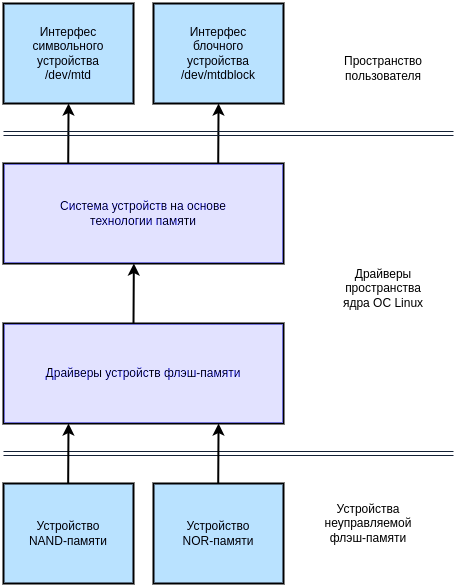
\includegraphics[scale=0.7]{mtd-noback.png}
	\caption{Подсистема устройств технологии памяти (MTD)}
	\label{mtdfigure}
\end{figure}

Она состоит из трех уровней: основной набор функций, драйверы микросхем флэш-памяти и драйверы пользовательского уровня, предоставляющие пользователю интерфейс символьного и блочного устройства для взаимодействия с флэш-памятью. 

\subsection{Устройства с несортированными блоками}

Подсистема \textbf{образов с несортированными блоками} (UBI - Unsorted Block Images) является частью модуля MTD. UBI предоставляет механизм абстракции над устройствами технологии памяти в виде томов, состоящих из логических стираемых блоков. Каждому логическому блоку соответствует физический стираемый блок усройства, при том соседние логические блоки необязательно будут связаны с соседними физическими блоками устройства. Помимо возможности разделения устройства на несколько томов, такая абстракция помогает избавить файловую систему от проблем обработки дефектных блоков устройства. Дефектные блоки находятся подсистемой UBI и не вклдючаются в томы. Механизм работы UBI продемонстрирован  на рис. ~\ref{ubifigure}.

\begin{figure}[H]
	\centering
	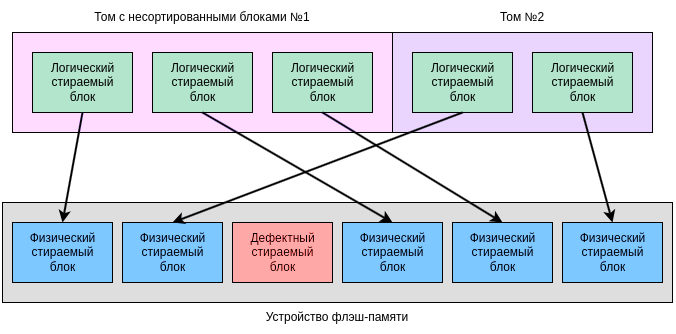
\includegraphics[scale=0.6]{ubi.png}
	\caption{Томы с несортированными блоками (UBI)}
	\label{ubifigure}
\end{figure}

Она состоит из трех уровней: основной набор функций, драйверы микросхем флэш-памяти и драйверы пользовательского уровня, предоставляющие пользователю интерфейс символьного и блочного устройства для взаимодействия с флэш-памятью. 

\subsection{Файловая система JFFS2}

Файловая система JFFS2 (Journaling Flash Filesystem 2) \cite{jffs2} была разработана для использования неуправляемых микросхем флэш-памяти в качестве запоминающего устройства и поддерживает устройства как NOR, так и NAND типа. JFFS2 является исторически первой файловой системой Linux для флэш-накопителей, но используется до сих пор. Она имеет журнальную структуру и использует подсистему устройств технологий памяти MTD для доступа к флэш-памяти.

Для того, чтобы избежать чтения всего журнала для вычисления структуры каталогов на этапе монтирования, JFFS2 использует сводные узлы (summary node). Сводный узел записывается в конец открытого стираемого блока и содержит в себе всю информацию, необходимую на этапе монтирования. Такой подход позволяет уменьшить время монтирования ценой небольшого перерасхода объема используемой памяти. Этот режим включается при установке определенного конфигурационного параметра ядра.

С целью различить является ли стираемый блок, в котором все биты установлены в 1 стертым, или он хранит полезную информацию, состояющую из всех единичных бит, JFFS2 использует маркеры очистки (clean marker), записываемые в начале блока. Если маркер очистки присутствует в блоке, значит блок очищен.

\subsection{Тестирования файловых систем}

Обеспечение надежности и отказоустойчивости модулей ядра, и файловой системы в частности - важная и непростая задача \cite{ostesting}. Наличие ошибок в исходном коде ФС может привести к нарушениям в основных функциях файловой системы, получению пользователем несанкционированного доступа к привелигированному режиму ядра, а также полному краху или блокировке системы. Подобные последствия ошибок на серверах и суперкомпьютерах могут привести к потерям значимых данных или несанкционированному доступу к ним.

Большинство веб-серверов и суперкомпьютеров используют операционные системы на основе ядра Linux, имеющего открытый исходный код. В ядре Linux имеется множество файловых систем, разработанных для различных типов устройств хранения информации и использующие различные алгоритмы расположения данных на устройстве. 

Решением для проверки корректности функционирования операционных систем и их модулей является создание систем автоматизированного тестирования.  

Важнейшей метрикой, характеризующей качество подобных систем тестирования является тестовое покрытие кода. Полнота тестового покрытия кода является предметом для множества исследований, в том числе в области тестирования файловых систем. В частности, в данной работе будет рассмотрена проблема создания системы автоматизированного тестирования файловой системы JFFS2, а также исследование достигаемого тестового покрытия исходного кода этой файловой системы.

\newpage
 %% Введение
    \section{Постановка задачи}
\label{sec:Chapter1} \index{Chapter1}

Целью данной работы является разработка системы автоматизированного тестирования файловой системы JFFS2.

Для достижения данной цели были поставлены следующие задачи:

\begin{itemize}
	\item Изучить особенности внутреннего устройства файловойсистемы JFFS2.
	\item Иследовать существующие решения тестирования файловых систем и модулей ядра Linux.
	\item Расширить тестовое покрытие кода, достигаемое существующими решениями.
	\item Разработать тесты, соответствующие особенностям JFFS2.
\end{itemize}

Актуальность данной работы обусловлена тем, что инструменты тестирования ядра Linux в лаборатории Linux Verification Center часто обнаруживают в исходном коде JFFS2 ошибки, требующие исправлений. Для проверки корректности внесенных исправлений требуется система тестирования, специализированная под особенности этой ФС и покрывающая своими тестами основной функционал.

JFFS2 в данный момент не имеет тестовых наборов, специализированных под ее архитектурные особенности ввиду небольшой популярности. Однако эта ФС до сих пор используется на множестве устройств.

\newpage
 %% Постановка задачи
    \section{Обзор существующих решений}
\label{sec:Chapter2} \index{Chapter2}

Для большинства файловых систем ядра Linux сообществом были разработаны тестовые наборы, фреймворки стресс-тестирования и инструменты фаззинг-тестирования. В данной главе будут описаны наиболее популярные и подходящие к тестированию JFFS2 решения.

\subsection{Xfstests}

\textbf{Xfstests} \cite{xfstests} - набор регрессионных тестов, изначально разработанный под файловую систему xfs, но в данный момент поддерживает множество других файловых систем ядра Linux, среди которых btrfs, reiserfs, f2fs и другие. Этот набор представляет собой множество bash-скриптов, разделенных по каталогам на группы. Среди тестов имеются как нацеленные на тестирование общих для всех ФС функций, так и предназначенные для определенных систем. На данный момент xfstests является наиболее популярным и широко использующимся решением для тестирования файловых систем.

\subsection{Fsfuzz}

\textbf{Fsfuzz} \cite{fsfuzz}- это инструмент фаззинг-тестирования ФС, представляющий собой bash-скрипт, суть работы которого заключается в генерации множества случайных образов выбранной файловой системы и дальнейшего монтирования этих образов. Подобный метод перебора не покрывает все основные функции файловой системы, однако может привести к редким сценариям обработчика ошибок, что полезно, так как подобные редкие сценарии сложно покрыть обычными тестовыми наборами.

\subsection{Syzkaller}

\textbf{Syzkaller} \cite{syzkaller} - наиболее популярный инструмент динамического анализа кода ядра ОС. Суть его работы заключается в конструировании случайных программ наоснове системных вызовов, запуске их на тестируемой системе и получении обратной связи в виде покрытия кода ядра. Случайные программы конструируются с использованием различных системных вызовов в различном порядке и со случайно подобранными аргументами с целью расширения покрытия кода. При достижении ошибок syzkaller генерирует программы репродьюсеры на языке Си, повторяющие сценарий достижения ошибки.

В файле конфигурации syzkaller можно определить список разрешенных к использованию системных вызовов, таким образом ограничить его покрытие, но нацелить на определенные сценарии с выбранными системными вызовами. При должной конфигурации syzkaller может быть использован для тестирования определенного модуля ядра, в том числе и ФС. 

\subsection{Тесты из пакета инструментов MTD}

Пакет \textbf{mtd-utils} \cite{mtd-utils} содержит множество инструментов для работы с устройствами флэш-памяти, в том числе и инструмент создания образа файловой системы JFFS2. Разработчиками этого пакета инструментов были добавлены тесты для файловых систем флэш-памяти в виде четырех bash-скриптов.

Эти тесты должны хорошо покрывать функции, отвечающие особенностям файловой системы JFFS2, однако такого небольшого числа скриптов недостаточно для покрытия всех основных функций ФС.

\newpage
 %% Обзор существующих решений
    \section{Исследование и построение решения задачи}
\label{sec:Chapter3} \index{Chapter3}

В данной главе будут подробно рассмотрены идеи, разработанные в ходе исследования и построения решения задачи. Реализации данных идей подробно описывается в следующей главе.

\subsection{Тестовое покрытие}

\textbf{Тестовое покрытие} является основной метрикой, характеризующей качество системы тестирования любой программы. Однако функционал модулей ядра операционной системы, и ФС в частности, во многом зависит от конфигурации окружения, в котором она работает. То есть для получения полной информации о покрытии достигаемом при помощи тестового набора необходимо провести несколько экспериментов в различном окружении.

\subsection{Расширение тестового покрытия ФС}

Для расширения тестового покрытия исходного кода ФС, достигаемого при помощи тестового набора, необходимо провести анализ основных функций тестируемой ФС и параметров конфигурации ее окружения, от которых зависит ее функционал.

\subsection{Функционал JFFS2}

Основные функции файловой системы JFFS2 можно разделить на несколько групп по их предназначению:

\begin{enumerate}
	\item \textbf{Основные операции с файлами.}

	К этой группе относятся функции, отвечающие за основной функционал операций с файлами, каталогами и внутренними структурами  ФС. Этот базовый функционал является общим для всех ФС. К таким операциям относятся чтение и запись данных в файл, создание и удаление файла или каталога и соответствующих им индексных дескрипторов, установка расширенных атрибутов файлов. Функции этой группы могут быть покрыты тестовыми наборами других ФС, так как являются частью общего для всей файловых систем функционала.

	\item \textbf{Функции контроля доступа.}

	К этой группе относятся функции, отвечающие за контроль доступа к пользовательским данным и операции с внутренними структурами, отвечающими за это, например, списком контроля доступа.

	\item \textbf{Функции взаимодействия с устройствами хранения.}

	К этой группе относятся функции, определяющие тип устройства хранения с которым работает ФС и работающие с его блоками, например, обеспечивающие выравнивание износа стираемых блоков.

	\item \textbf{Сборщик мусора.}

	Эта группа включает в себя функции, обеспечивающие работу алгоритма сборщика мусора JFFS2. Этот алгоритм является специфичным для этой ФС и его функции могут не покрываться при стандартных сценариях.

	\item \textbf{Алгоритмы сжатия данных.}

	В JFFS2 есть 4 различных алгоритма сжатия данных, состоящих из множества внутренних функций. Помимо функционала самих алгоритмов, в коде присутствуют функции, отвечающие за стратегию выбора алгоритма сжатия. Например, выбор может производиться по приоритету, размеру сжатых данных или вынуждая ФС в любом случае использовать один алгоритм.

	\item \textbf{Обработчики ошибок.}

	К этой группе относятся функции, обрабатывающие ошибки и редко достигаемые в обычных сценариях работы ФС. Эти ошибки могут быть связаны с некорректным выделением памяти, несоответствием важных параметров образа и устройства, используемого для его подключения или невалидностью данных, по причине наличия ошибок во внутренней логике самой файловой системы. Функции этой группы лучше всего покрываются при помощи \textbf{фаззинг-тестирования}, либо тестированием с \textbf{симуляцией сбоев}.

	\item \textbf{Обработка входных параметров команд.}

	К этой группе относятся функции, обрабатывающие суперблок ФС и входные параметры при выполнении команды монтирования. Эти функции являются частью основного функционала любой ФС, однако могут быть выделены в отдельную группу, так как лучше покрываются фаззинг-тестированием ввиду большой вариативности возможных входных параметров и образа ФС.

	\item \textbf{Функции работы с внутренними структурами.}

	К этой группе относятся функции, работающие со внутренними структурами, особенными для исследуемой ФС. Для JFFS2 такими структурами являются, например, сводные узлы и маркеры очистки блоков. Ввиду своего назначения, эти функции могут не покрываться обычными тестовыми наборами и требовать написания специализированных тестов.
\end{enumerate}

\subsection{Окружение файловой системы}

Функционал файловой системы зависит от множества параметров ее окружения. В данном разделе будут выделены факторы, от которых зависит функционал JFFS2.

Во-первых, для различных типов запоминающих устройств файловая система может использовать разные функции для работы с данными. Файловая система jffs2 по разному работает с устройствами технологии памяти типа NOR и NAND, а также имеет особый интерфейс взаимодействия с образами с несортированными блоками (UBI) \cite{ubi} и устройствами флэш-памяти dataflash, подключаемыми по шине SPI. 

Во-вторых, при тестировании заранее созданного образа ФС, тестируемый образ может быть создан с различными опциями. Для файловой системы JFFS2 опции команды mkfs, создающей образ ФС, могут быть использованы для задания размера выходного образа, размера стираемого блока, размера страницы, используемого алгоритма сжатия данных, используемой стратегии автоматического выбора алгоритма сжатия, используемого порядка бит в выходном образе и подключения, либо отключения функционала расширенных атрибутов файлов Linux. 

В-третьих, при тестировании команды монтирования, используемой для подключения файловой системы к единому дереву каталогов, могут быть указаны различные опции. При помощи опций общих для всех файловых систем можно устанавливать режим доступа к данным, содержащимся на подключаемом устройстве, например, доступ только для чтения, либо для чтения и записи. С использованием опций специфичных для JFFS2 можно, например, выбрать используемый алгоритм сжатия данных.

В-четвертых, функционал собранного ядра операционной системы во многом определяется составленным на этапе сборки файлом конфигурации. Опции, определяемые в этом файле могут отвечать за подключение определенных модулей ядра и указание параметров для этих модулей. Для модуля устройств на основе технологии памяти в конфигурационном файле могут быть указаны опции, отвечающие за подключение различных эмуляторов и определение их параметров, поддержку драйверов нужных для взаимодействия с различными чипами и контроллерами устройств памяти. Для файловой системы JFFS2 при помощи опций конфигурационного файла подключается поддержка расширенных атрибутов Linux, поддержка буфера записи, использование структуры сводных узлов и маркеров очистки и поддержка различных алгоритмов сжатия. Также при помощи конфигурационных опций может быть выбрана стратегия автоматического выбора алгоритма сжатия. Например, строка "CONFIG\_JFFS2\_CMODE\_PRIORITY=y"\ в файле конфигурации ядра указывает файловой системе выбирать алгоритм сжатия на основе их приоритета, а строка "CONFIG\_JFFS2\_CMODE\_SIZE=y"\ указывает на выбор алгоритма сжатия на основе размера сжатых данных.

\subsection{Создание системы автоматизированного тестирования}

В соответствии с целью и поставленными в работе задачами, для создания системы автоматизированного тестирования файловой системы JFFS2 необходимо протестировать исследуемую ФС при помощи имеющихся решений, в процессе доработать или адаптировать необходимые инструменты, расширить покрытие, достигаемое при использовании имеющихся решений, произведя запуск в различных конфигурациях окружения, протестировать функции обработки ошибок при помощи инструментов фаззинг-тестирования, и создать тесты, покрывающие редкие сценарии, с использованием технологии внедрения ошибок.

\newpage
 %% Исследование и построение решения задачи
    \section{Описание практической части}
\label{sec:Chapter4} \index{Chapter4}

\subsection{Использованные инструменты}

В данном разделе будет приведен список инструментов используемых в ходе практической части работы.

В ходе всей работы по тестированию JFFS2 используется код ядра Linux версии 5.10 из репозитория \cite{lvcrepo} лаборатории Linux Verification Center. Процесс тестирования происходит на виртуальной машине Qemu, эмулирующей машину архитектуры x86-64 под гостевой системой Ubuntu Linux.

Для тестирования сценариев работы с различными типами устройств флэш-памяти без использования реальных микросхем памяти, необходимо использовать эмуляторы флэш-устройств. На данный момент в модуле устройств на основе технологии памяти (MTD) \cite{mtd} ядра Linux реализованы 3 эмулятора: mtdram, эмулирующий NOR-память в оперативной памяти системы, block2mtd, эмулирующий устройство NOR-памяти поверх блочного устройства и nandsim, эмулирующий устройство NAND-памяти в оперативной памяти. Поддержка эмуляторов подключается в файле конфигурации ядра, например параметр "CONFIG\_MTD\_MTDRAM"\ отвечает за использование эмулятор mtdram, а параметры "CONFIG\_MTDRAM\ \_TOTAL\_SIZE"\ и "CONFIG\_MTDRAM\_ERASE\_SIZE"\ устанавливают размер эмулируемого устройства и размер его стираемого блока.

За основу при создании системы автоматизированного тестирования было решено взять тестовый набор xfstests, так как он содержит в себе множетсво скриптов, тестирующих базовые функции общие для всех ФС, а также является наиболее популярным решением для тестирования файловых систем ядра Linux и имеет удобный функционал для добавления новых тестов. Для добавления в набор xfstests своих тестовых сценариев необходимо описать сценарий в виде bash-скрипта, запустить скрипт new для добавления нового теста в набор и создать файл, определяющий выходные данные, которые должны генерироваться в ходе корректной работы теста. При тестировании xfstests использует 2 блочных устройства, называющиеся TEST и SCRATCH с тестируемой ФС на них и два каталога, используемые для монтирования. Для предоставления тестовому набору интерфейса блочного устройства в модуле MTD есть драйвер mtdblock. Для использования этого драйвера необходимо установить соответсвующую ему опцию конфигурацияи ядра, что делается при помощи строки  "CONFIG\_MTD\_BLOCK=y".

Для сбора ирнформации о покрытии исходного кода модулей ядра используется утилита gcov \cite{gcov}. Для визуализации собранной информации в виде html отчета используется расширение утилиты gcov - lcov \cite{lcov}. Для сбора информации о покрытии в ядре Linux достаточно установить параметр конфигурации ядра "CONFIG\_GCOV\_KERNEL"\ при его сборке, а так же параметр "GCOV\_PROFILE"\ в файле сборки модуля fs/jffs2/Makefile для активации профилирования директории,содержащей исходные файлы тестируемой ФС. Для сбора корректного покрытия в ходе работы тестов перед запуском необходимо сбросить информацию о покрытии. Сброс покрытия можно осуществить командой  "echo 0 > /sys/kernel/debug/gcov/reset". После окончания работы тестов, информация о покрытии хранится в директории /sys/kernel/debug/gcov. На основе собранного покрытия утилита lcov генерирует информационный файл, который преобразуется в html-отчет утилитой genhtml.

Для создания тестируемого образа файловой системы используется команда mkfs с опцией определяющей тип файловой системы. Команда для создания образа JFFS2 (mkfs.jffs2) является частью пакета инструментов для работы с флэш-памятью mtd-utils \cite{mtd-utils}. По неизвестной причине, из четырех алгоритмов сжатия, поддерживаемых JFFS2, команда создания образа файловой системы поддерживала только 3: lzo, zlib и rtime. С целью достичь более полного тестирования исходного кода, в процессе работы исходный код инструмента mkfs.jffs2 был доработан, и таким образом была добавлена возможность создания образа JFFS2 с использованием алгоритма сжатия rubin.

Как было описано в прошлой главе, JFFS2 имеет специальные функции для работы с устройствами dataflash, подключенными по пртоколу SPI и устройствами разделенными на томы с несортированными блоками (UBI устройства) \cite{ubi}. К сожалению в открытом доступе нет эмулятора устройства dataflash, для тестирования сценария монтирования устройства такого типа, однако в модуле MTD есть эмулятор устройств с несортированными блоками - gluebi. Для подключения этого эмулятора в конфигурационном файле ядра используется строка "CONFIG\_MTD\_UBI\_GLUEBI=y". Подсистема UBI, являющаяся частью модуля MTD выполняет функции уровня флэш-преобразования, обеспечивая выравнивание износа блоков устройства, а также управляет томами, являющимися более высокоуровневой абстракцией над устройствами технологии памяти. В процессе практической работы, эмулятор gluebi вызывал панику ядра путем разыменования нулевого указателя. Для корректного использования эмулятора потребовалось исправление его исходного кода.

Для покрытия функций обработки ошибок фаззинг-тестированием, в работе будут использованы инструменты syzkaller \cite{syzkaller} и fsfuzz \cite{fsfuzz}. Не смотря на то, что в документации инструмент фаззинг-тестирования файловых систем fsfuzz заявляется о совместимости с файловой системой JFFS2, прямолинейный запуск инструмента для исследуемой ФС не принес результата, так как bash-скрипт fsfuzz использует при монтировании виртуальные блочные устройства, что является неподходящим для JFFS2. После внесения правок в исходный код инструмента с целью использования MTD устройств при указании в качестве опции тип файловой системы JFFS2, инструмент удалось применить к тестированию исследумой ФС.

Для симуляции сбоев во внутренних функциях модуля ФС в работе будет применен встроенный в ядро Linux инструмент Linux Fault Injection \cite{fault}. Этот инструмент позволяет симулировать сбои почти всех функций ядра, предоставляя пользователю возможность установить в качестве параметров вероятность ошибки, интервал между сбоями, их количество и возвращаемое функцией значение. Для симуляции сбоя функции необходимо разрешить в коде ядра внедрение неисправности в эту функцию при помощи макроса ALLOW\_ERROR\_INJECTION. Сам инструмент можно использовать при установке параметра конфигурации ядра "CONFIG\_ FAULT\_INJECTION".

\subsection{Тестирование с использованием готовых решений}

Для тестирования файловой системы с использованием готовых решений необходима предварительная сборка ядра с определенной конфигурацией, наличие тестируемого образа файловой системы и блочных устройств для монтирования. Далее в этом разделе будет описана базовая конфигурация, необходимая для тестирования JFFS2 при помощи готовых решений.

Во первых, необходимо в конфигурации ядра добавить поддержку тестируемой ФС и необходимой для ее работы подсистемы устройств технологии памяти, которая отсутствует в базовой конфигурации ядра. Это может быть осуществлено добавлением следующих строк в файл конфигурации ядра Linux: "CONFIG\_MTD=y"\ - подключение подсистемы MTD, "CONFIG\_JFFS2\_FS=y"\ - подключение модуля JFFS2. Во-вторых, после конфигурации и сборки ядра необходимо создать образ тестируемой ФС. Для этого используется команда mkfs.jffs2, являющаяся частью пакета инструментов mtd-utils, который требует предварительной установки, например при помощи менеджера пакетов apt-get. В третьих, для монтирования тестируемой ФС необходимы блочные устройства, которые в случае JFFS2 создаются драйвером mtdblock поверх MTD устройств эмулируемых одним из эмуляторов, например block2mtd, который тоже необходимо подключить в конфигурации ядра.

\subsection{Результаты первого эксперимента}

Прямолинейный запуск набора xfstests в совокупности с тестами из пакета mtd-utils в описаной выше минимальной необходимой конфигурациидал результат в виде тестового покрытия исходного кода в 64\% исходного кода. Следующим важным шагом является расширение тестового покрытия, на основе анализа функционала JFFS2 и параметров окружения, который был приведен в прошлой главе, а также анализа достигнутого в первом эксперименте покрытия.

\subsection{Расширение тестового покрытия}

Первым шагом на пути к расширению тестового покрытия является добавление в конфигурации ядра всего функционала тестируемой ФС. Опции конфигурации JFFS2 и функционал на который они влияют описаны в файле fs/jffs2/Kconfig.

Анализ достигнутого при первом эксперименте покрытия показал, что не покрыты функции, используемые для работы с устройствами NAND-памяти и UBI томами, так как используемые эмулятор block2mtd эмулирован флэш-память NOR-типа. Для расширения тестового покрытия необходимо использовать эмулятор UBI томов gluebi и NAND-памяти nandsim.

Также не были покрыты функции алгоритмов сжатия данных. Для их покрытия необходимо подключить их поддержку в конфигурации ядра, создать несколько тестируемых образов с разными параметрами mkfs, например команда "mkfs.jffs2 \-\-compression-mode=size"\ создает образ ФС, алгоритм сжатия на котором будет определяться размерам сжатых данных. Для использования каждого конкретного алгоритма сжатия можно установить режим выбора алгоритма на выбор по приоритету и устанавливать приоритет тестируемого алгоритма выше остальных параметрами команды mkfs. Например команда "mkfs.jffs2 \-\-compression-priority=100:zlib"\ устанавливает максимальный приоритет алгоритму zlib.

\subsection{Расширенное тестовое покрытие}

Тестовые наборы были перезапущены несколько раз с различными конфигурациями. Покрытия полученные в этих экспериментах, объединенные с результатом первого эксперимента дали результат в виде тестового покрытия в 75.8\%.

По сравнению с первым экспериментом тестовое покрытие увеличилось на 11.8\% или на 1275 строк кода.

\subsection{Фаззинг-тестирование}

Наиболее популярный инструмент фаззинг-тестирования ядра Linux и его модулей - syzkaller. Однако он плохо подходит для задачи тестирования файловой системы, так как суть его работы заключается в генерации случайных программ состоящих из различных системных вызовов. Для достижения типичного сценария работы ФС syzkaller должен сгенерировать программу, состоящую как минимум из монтирования валидного образа файловой системы и дальнейших взаимодействий с ним при помощи, например системных вызовов open, write и close. Для случайной генерации подходящего сценария потребуется множество перебранных неудачных вариантов последовательностей системных вызовов или монтирования невалидных образов.

Для того, чтобы сузить тестируемые syzkaller области, был применен файл конфигурации, приведенный в ПРИЛОЖЕНИИ. Параметры конфигурации syzkaller указывают ему список разрешенных к использованию системных вызовов и запрещают другие, чтобы он быстрее приходил к нужному сценарию. Инструменты описания грамматики системных вызовов, разработанные в syzkaller позволяют определить свою "мутацию" системного вызова заключающуюся например в определенных передаваемых параметрах. Таким образом в файле sys/linux/filesystem.txt определен системный вызов монтирования образа файловой системы JFFS2: "syz\_mount\ \_image\$jffs2". При включении этого вызова в конфигурации и отключении других вариантов монтирования, монтирование всего будет производиться с параметром типа файловой системы jffs2.

При столкновении с ошибкой в виде блокировки, неопределенного поведения, либо просто сообщения об ошибке или предупреждения syzkaller генерирует программу репродьюсер на языке Си, при запуске которой будет вопроизведен сценарий достигающий этой ошибки. Для генерации репродьюсеров при достижении определенной строки нужно добавить в коде ядра генерацию предупреждения об ошибке при достижении этой строки, что можно реализовать например при помощи макроса "WARN\_ON(1)".

При помощи syzkaller удалось достичь покрытия 11 ранее непокрытых строк, отвечающих редким сценариям при обработке суперблока в процессе монтировании ФС.

Таким образом для расширения покрытия кода ФС, syzkaller был запущен в конфигурации, разрешающей ему производить только системные вызовы для работы с ФС. Достигаемое им тестовое покрытие было проанализировано и в недостижимые ранее строки были помещены предупреждения об ошибках. При повторном запуске syzkaller при достижении этих строк он генерировал программы репродьюсеры, которые необходимо добавить в разрабатываемую систему автоматизированного тестирования.

При тестировании JFFS2 при помощи доработанного инструмента фаззинга файловых систем fsfuzz было также достигнуто покрытие 13 ранее непокрытых строк, составляющих две ранее непокртые функции обновления опций монтирования при реконфигурации суперблока ФС.

Таким образом, фаззинг-тестирование помогло покрыть 24 ранее непокрытых строки кода, достижимые только при редких случаях работы ФС.

\subsection{Тестирование с использованием симуляции сбоев}

Исходном код модулей ядра Linux и ФС в частности содержат множество строк кода, отвечающих за обработку крайне редко происходящих сценариев, которые однако в случае возникновения должны быть корректно обработаны. Наглядным примером подобных обработчиков ошибок, редко встречаемых в типичном сценарии работы модуля, является проверка значения, возвращаемого функциями выделения памяти. Для тестирования корректной работы ядра в подобном сценарии используется технология симуляции сбоев \cite{faultuse}.

В данной работе применялся метод целенаправленной разработки тестов с симуляцией сбоев, который малоэффективен при создании универсальной системы тестирования нескольких модулей или драйверов ядра, однако подходит для создания тестов направленных на работу с определенной файловой системой.

При анализе тестового покрытия был обнаружен достаточно большой участок кода, обрабатывающий сценарий сбоя в функции записи данных на флэш-память jffs2\_flash\_writev. Соседние этому обработчику ошибки строки покрываются тестом номер 3 из группы generic из набора xfstests. 

Для симуляции сбоя в этой функции был использован инструмент Linux Fault Injection, функционал которого можно подключить, определив в файле конфигурации ядра параметр "CONFIG\_FAULT\_INJECTION".\ В параметрах внедрения ошибок было указано имя функции, в которой по тестовому сценарию должен произойти сбой, единичный интервал между сбоями, вероятность сбоя 100\%, количество сбоев равное количеству запуска тестируемой функции в рассматриваемом тесте набора и возвращаемое значение функции -12, соответствующее коду ошибки в случае отсутствия свободной памяти (-ENOMEM).

При запуске выбранного теста с использованием симуляции сбоя функции jffs2\_flash\_writev удалось покрыть 24 ранее непокрытые строки обработки ошибки в запускающей ее функции jffs2\_write\_dnode, а также ранее непокрытую функцию проверки корректности суперблока ФС в случае подобной ошибки, состояющую из 5 строк кода. Кроме того дополнительно были покрыты 7 строк обрабатывающие ошибку произошедшую в функции jffs2\_write\_dnode. Таким образом тест с использованием симуляции сбоя во внутренней функции JFFS2 покрывает 36 ранее непокрытых строк.

Аналогичным образом был создан второй тест, на основе того же теста из набора xfstests, покрывающий при помощи симуляции ошибки в функции создания нового индексного дескриптора по причине нехватки памяти. Данный тест покрывает 3 новые строки кода функции jffs2\_create.

\subsection{Анализ непокрытого кода}

Суммарное покрытие, достигаемое тестами из набора xfstests и пакета mtd-utils, тестами, созданными из программ репродьюсеров сгенерированных инструментом syzkaller и фаззинг-тестирования при помощи fsfuzz составляет 6216 строк кода из 7829, что соответствует покрытию 79.4\% строк исходного кода. Функциональное покрытие составляет 91.4\% или 286 из 313 функций. При достижении подобного результата дальнейшее увеличение тестового покрытия кода является крайне трудоёмкой задачей и покрытие 79.4\% строк кода можно считать достойным результатом. Однако каждая функция добавляется в код ФС для выполнения особой задачи, и факт наличия непокрытых функций является проблемой, так как тестовые скрипты не соответствуют всем возможным сценариям работы файловой системы.

Для дальнейшего развития системы тестирования исследуемой файловой системы и подведения итогов проделанной работы необходимо провести анализ непокрытого кода.

Оставшиеся непокрытыми 27 функций были классифицированы на 4 группы. Результат представлен на рис. ~\ref{funcs}.

\begin{figure}[H]
	\centering
	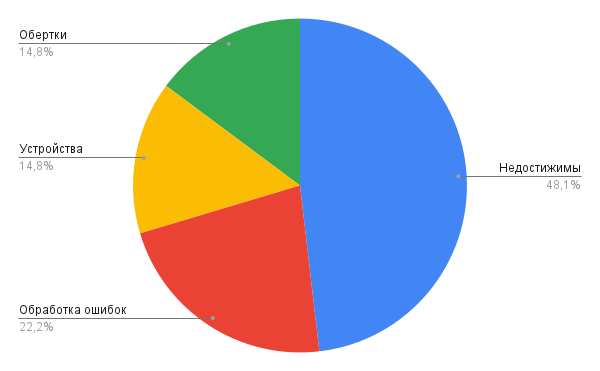
\includegraphics[scale=0.75]{chart.png}
	\caption{Катеогории непокрытых функций}
	\label{funcs}
\end{figure}

Во-первых, 13 из этих функций можно считать недостижимыми при подходе тестирования скриптами пространства пользователя. Наглядным примером являются функции деинициализации алгоритмов сжатия. Деинициализация структур, хранящих данные об алгоритмах сжатия, происходит в случае возникновении ошибки при инициализации модуля ФС, что происходит на этапе загрузки ядра ОС. Внедрить ошибки для тестирования подобного сценария невозможно используя скрипты пространства пользователя.

Во-вторых, 6 функций отвечают за обработку ошибок в редких сценариях и могут быть покрыты при помощи специальных тестов с использованием симуляции сбоев, аналогично тестам, описаным в прошлом разделе.

В-третьих, 4 непокрытых функций нужны для работы ФС с особыми видами устройств флэш-памяти. Например функция jffs2\_dataflash\_setup и jffs2\_dataflash\_cleanup выполняют соответственно инициализацию и деинициализацию буффера записи, для работы с устройством dataflash. Еще 2 функции имеют такое же назначение, но для работы с NOR-памятью с контроллером.

В-четвертых, 4 функции отвечают за операции с суперблоком файловой системы, как например поиск родительского каталога. Эти функции могут быть покрыты тестами пользовательского пространства, однако они фактически являются обертками над функциями, которые являются общими для всех ФС и определены вне директории модуля JFFS2. Как например функция jffs2\_fh\_to\_parent просто ссылается на функцию generic\_fh\_to\_parent, определенную в файле fs/libfs.c.

\newpage
 %% Описание практической части
    \section{Заключение}
\label{sec:Chapter5} \index{Chapter5}

В результате проделанной работы была разработана система автоматизированного тестирования файловой системы JFFS2 на основе существующих решений для тестирования файловых систем. В процессе разработки системы тестирования был доработан инструмент создания образа JFFS2, путем добавления в него поддержки алгоритма сжатия данных rubin, с использованием драйвера mtdblock был адаптирован под особенности JFFS2 инструмент фаззинг-тестирования файловых систем fsfuzz. 

Набор xfstests, являющий наиболее популярным и поддерживаемым сообществом пользователей и разработчиков Linux решением для тестирования файловых систем, был адаптирован с целью тестирования JFFS2. К существующим тестовым скриптам набора были добавлены тесты пакета mtd-utils, тесты созданные из программ сгенерированных инструментом syzkaller и тесты, использующие симуляцию сбоев внутренних функций JFFS2.

Разработанная система тестирования была экспериментально проверена. В результате проведённого тестирования всеми полученными скриптами было достигнуто покрытие в 79,4\% строк исходного кода и 91,4\% функций. Это является достойным результатом и дальнейшее расширение тестового покрытия является крайне сложной задачей.

С целью дальнейшего развития разработанной системы был произведен анализ достигаемого тестового покрытия исходного кода, в результате которого были классифицированы непокрытые тестами функции ФС. По итогу проведенного анализа выявлено, что 48\% непокрытых функций являются недостижимыми при тестировании скриптами пользовательского пространства. Для тестирования еще 15\% непокрытых функций необходимо использование реальных устройств флэш-памяти определенного типа, ввиду отсутствия эмуляторов. В тестирование еще 15\% непокрытых функций нет острой необходимости, так как они фактически являются обертками над функциями общей для всех ФС библиотеки, которые могут быть протестированы другими тестовыми наборами. И оставшиеся 22\% непокрытых функций, что эквивалентно 2\% от общего числа функций файловой системы могут быть покрыты при дальнейшем развитии тестовой системы. 

Дальнейшее увеличение тестового покрытия является трудоёмкой задачей, но важно продолжать работу над улучшением качества тестирования, чтобы обеспечить более полное покрытие кода и повысить надёжность файловой системы.

\newpage
 %% Заключение

    %% НЕ ТРОГАЙТЕ!!!
    \nocite{*}
    \bibliography{references}

    %% в зависимости от надобности подключаем раздел "Приложение"
    \newpage
    \section*{Приложение А}
\addcontentsline{toc}{section}{Приложение А}
\label{sec:Apendix} \index{Apendix}

\section*{Полная конфигурация ядра}


CONFIG\_MTD=y

CONFIG\_MTD\_BLKDEVS=y

CONFIG\_MTD\_BLOCK=y

CONFIG\_MTD\_MTDRAM=y

CONFIG\_MTDRAM\_TOTAL\_SIZE=8192

CONFIG\_MTDRAM\_ERASE\_SIZE=128

CONFIG\_MTD\_BLOCK2MTD=y

CONFIG\_MTD\_NAND\_CORE=y

CONFIG\_MTD\_NAND\_NANDSIM=y

CONFIG\_MISC\_FILESYSTEMS=y

CONFIG\_JFFS2\_FS=y

CONFIG\_JFFS2\_FS\_WRITEBUFFER=y

CONFIG\_JFFS2\_FS\_WBUF\_VERIFY=y

CONFIG\_JFFS2\_SUMMARY=y

CONFIG\_JFFS2\_FS\_XATTR=y

CONFIG\_JFFS2\_FS\_POSIX\_ACL=y

CONFIG\_JFFS2\_FS\_SECURITY=y

CONFIG\_JFFS2\_COMPRESSION\_OPTIONS=y

CONFIG\_JFFS2\_ZLIB=y

CONFIG\_JFFS2\_LZO=y

CONFIG\_JFFS2\_RTIME=y

CONFIG\_JFFS2\_RUBIN=y

\# CONFIG\_JFFS2\_CMODE\_NONE is not set

CONFIG\_JFFS2\_CMODE\_PRIORITY=y

\# CONFIG\_JFFS2\_CMODE\_SIZE is not set

\# CONFIG\_JFFS2\_CMODE\_FAVOURLZO is not set

    \newpage
    \section*{Приложение Б}
\addcontentsline{toc}{section}{Приложение Б}
\label{sec:Apendix} \index{Apendix}

\section*{Конфигурация syzkaller}

\{

        "target"\ : "linux/amd64"\ ,

        "http"\ : "127.0.2.1:56741"\ ,

        "workdir"\ : "syzkaller/workdir"\ ,

        "kernel\_obj"\ : "linux-stable"\ ,

        "image"\ : "syzkaller/tools/bullseye.img"\ ,

        "sshkey"\ : "syzkaller/tools/bullseye.id\_rsa"\ ,

        "syzkaller"\ : "syzkaller"\ ,

        "procs"\ : 2,

        "type"\ : "qemu"\ ,

        "vm"\ : \{

                "count"\ : 1,

                "cpu"\ : 2,

                "mem"\ : 8096,

                "kernel"\ : "linux-stable/arch/x86/boot/bzImage"\ ,

                "cmdline"\ : "net.ifnames=0"\ 

        \},

        "interests"\ : ["fs/jffs2/"\ ],

        "enable\_syscalls"\ : ["syz\_mount\_image\$jffs2"\ ,\ "getuid"\ , "geteuid"\ , 

                "fstat"\ , "getresuid"\ , "open"\ , "write"\ , "read"\ ]

\}

\end{document}
